\section{Results}

\subsection{Skeleton Pruning}

\paragraph{Finding Positive Examples.}

As a baseline, we consider all pairs of segments that have neighboring voxels and see what percent of these segments are considered for merging. In the L. Cylinder dataset, there are XXX neighboring segments which have at least adjacent voxels. Our method which uses skeletons to prune the considered candidates finds XXX of these segments, or XX\% percent. On the FlyEM dataset, there are XXX adjacent segments with XXX found (XX\% percent). Figure \ref{fig:skeleton-results} shows some of the missed examples. The most common errors are the dendrite spines where the larger segment did not have an endpoint near the split. However, our algorithm does not require segments to be adjacent to merge. This offers a great benefit compared to traditional methods. In our datasets XXX and XXX segments are candidates for merging despite not having adjacent voxels. Figure \ref{fig:skeleton-results} gives one such pair which is merged given the results of our algorithm. 

\paragraph{Pruning Negative Examples.}

Traditional agglomeration strategies consider a large number of negative candidates that we hope to prune. The original approach of considering adjacent supervoxels has XX,XXX and XX,XXX candidates which do not belong to the same neuron. With our pruning algorithm, this reduces to X,XXX and X,XXX, a factor of over XX times. This allows a more reasonable training environment with greater balance between the positive and negative merge examples. 

\begin{figure}[t]
	\centering
	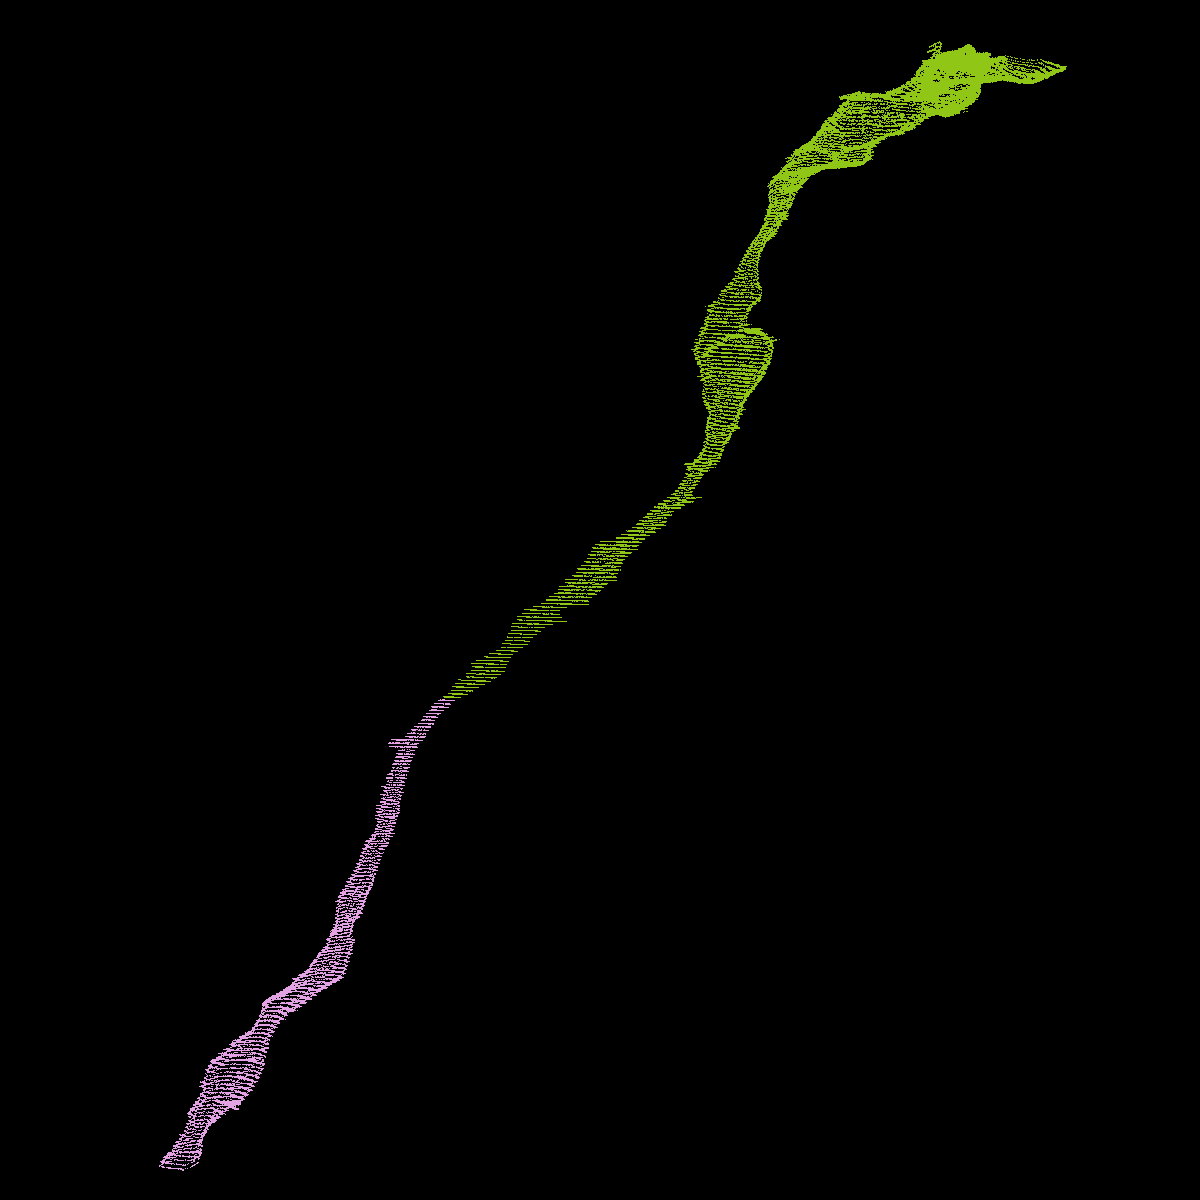
\includegraphics[width=0.42\linewidth]{./figures/merge_candidate1.png}
	\hspace{0.085\linewidth}
	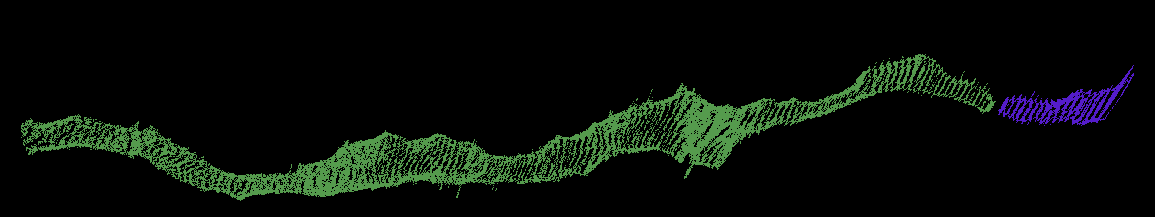
\includegraphics[width=0.42\linewidth]{./figures/merge_candidate2.png}
	\caption{Two erroneously split segments that should merge together. Most segments that we want to merge have the same general structure.}
	\label{fig:skeleton-results}
\end{figure}


\subsection{Classification Performance}

\begin{table}
	\centering
	\begin{tabular}{c c c c} \hline
	\textbf{Dataset} & \textbf{Precision} & \textbf{Recall} & \textbf{Accuracy} \\ \hline
	Kasthuri Training & & & \\
	Kasthuri Testing & & & \\
	FlyEM Vol. 1 & & & \\
	FlyEM Vol. 2 & & & \\ \hline
	\end{tabular}
	\caption{Precision and recall for the training and three test datasets.}
	\label{fig:classification}
\end{table}

Table \ref{table:classification} shows the precision and recall for all of the datasets. Our methods are more general than traditional connectomics examples allowing us to train the network on an anisotropic dataset and get impressive results on an isotropic dataset. Our initial network does not take in any image data, only the segment shapes, so we merely extract the $1200 \textrm{nm}^3$ region from any dataset and rescale as input into the neural network. For each of the tables, the top left square gives the number of segments which should merge that we predict merge. The bottom right square gives the number of segments which should not merge that we predict should not merge. The bottom left quadrant indicates the amount of false positives, candidates which we predict merge which do not. The top right quadrant gives the amount of false negatives where we predict split although the candidates should merge. Figure \ref{fig:network-results} shows the receiver operating characteristic (ROC) curve for all four datasets. 

\begin{figure}
	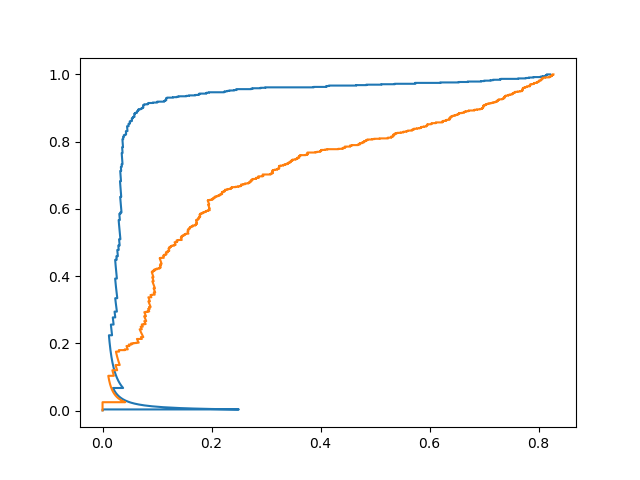
\includegraphics[width=0.9\linewidth]{./figures/roc-microns-300-test.png}
	\caption{The receiver operating characteristic (ROC) curve for all four datasets.}
	\label{fig:network-results}
\end{figure}

\subsection{Graph Based Strategies}

Using a graph-based optimization strategy prevents XX segments from merging compared to the simple hierarchical agglomeration strategy with an optimal threshold cut off. Since correcting merge errors is significantly more difficult than correcting split errors, it is desirable to limit the number of false merges. The graph-based strategies significantly improve this error type. 

\subsection{Variation of Information Improvements}

The final metric for comparing two connectomics segmentations is computing the variation of information with respect to an expert-labeled ground truth dataset. Figure \ref{fig:variation-of-information} shows the results on the datasets compared to the baseline (green) and an oracle (blue). 

\begin{figure*}[t!]
	\centering
	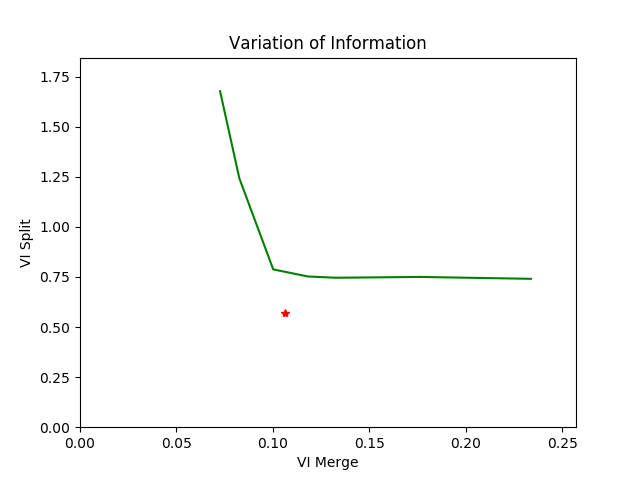
\includegraphics[width=0.42\linewidth]{./figures/variation_of_information-train.png}
	\hspace{0.085\linewidth}
	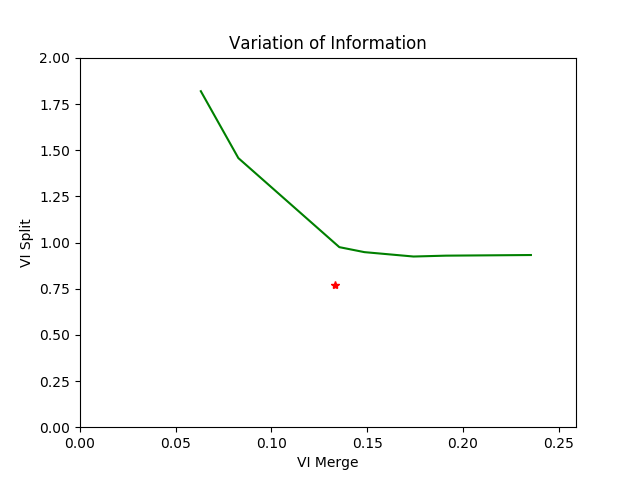
\includegraphics[width=0.42\linewidth]{./figures/variation_of_information-test.png}
	\caption{The improvement on variation of information from the baseline NeuroProof segmentation (green). Results closer to the origin are better.}
	\label{fig:variation-of-information}
\end{figure*}